\documentclass[letterpaper,11pt]{article}

\usepackage{fullpage,amsmath,amsfonts,latexsym,xcolor,clrscode3e}
\usepackage{graphicx}
\usepackage{amsthm}
\usepackage{hyperref}
\usepackage{fullpage}
\usepackage[ruled,vlined,linesnumbered]{algorithm2e}

\usepackage{subcaption}
\usepackage{caption}

\graphicspath{ {./images/} }

\newcommand{\re}{{\mathbb{R}}}
\newcommand\numberthis{\addtocounter{equation}{1}\tag{\theequation}}
\newcommand{\floor}[1]{\lfloor {#1} \rfloor}
\newcommand{\ceil}[1]{\lceil {#1} \rceil}
\newcommand{\paren}[1]{\left( {#1} \right)}
\newenvironment{solution}{\color{black} }{}

\newcommand{\nats}{\mathbb{N}}

\newcommand{\comment}[1]{$\rhd$\ {\small\sf #1}}

\newtheorem{theorem}{Theorem}
\newtheorem{claim}[theorem]{Claim}
\newtheorem{lemma}[theorem]{Lemma}
\newtheorem{problem}{Problem}


%\begin{document}
%{\noindent\large
%{\em Introduction to Analysis of Algorithms} \hfill \today\\
%Boston University \hfill CS 330\\
%Professor  Adam Smith, Dora Erdos \hfill Fall 2020\\}
%\vspace{1pt}
%\hrulefill\vspace{3mm}
%\begin{center}
%{\LARGE\bf Programming Assignment 1}\\
%{\bf Due October 24, 2020 at 11:59 PM}
%\end{center}
%
%\begin{center}
%   Student: Justin DiEmmanuele
%\end{center}


\begin{document}
\section{Grid Graph Analysis}
    \subsection{$G^{1}_{gr}$ and $G^{4}_{gr}$ Infected Nodes and Probability Distribution}

    For the two grid graphs, the infected node count is shown below for each 
    probability level.

    \begin{table}[htpb]
        \centering
        \caption{Count of Infected Nodes}
        \label{tab:infected_nodes}
        \begin{tabular}{c | c | c}
        p & $G^{1}_{gr}$ & $G^{4}_{gr}$ \\ 
        \hline
        0.1 & 28 & 56 \\ 
        0.3 & 310 & 417 \\ 
        0.5 & 1024 & 1024 \\
        0.7 & 1024 & 1024 \\
        \end{tabular}
    \end{table}

    $G^{4}_{gr}$, the grid graph with four infected source nodes, has clearly
    higher infection rates in the 0.1 and 0.3 probability levels. At 0.5 and 
    above, however, both graphs have a significant probability of infection for 
    all 1024 nodes. The following figures show the probability distributions 
    for both graphs.

    \begin{figure}[htpb]
        \centering
    \begin{subfigure}{.5\textwidth}
        \centering
        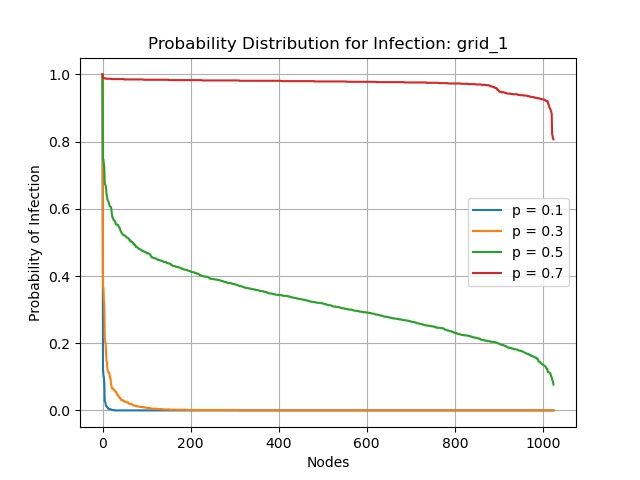
\includegraphics[width=0.9\textwidth]{pdist_grid_1.jpg}
        \caption{Probability Distributions $G^{1}_{gr}$}
        \label{fig:pdist_grid_1-jpg}
    \end{subfigure}%
    \begin{subfigure}{.5\textwidth}
        \centering
        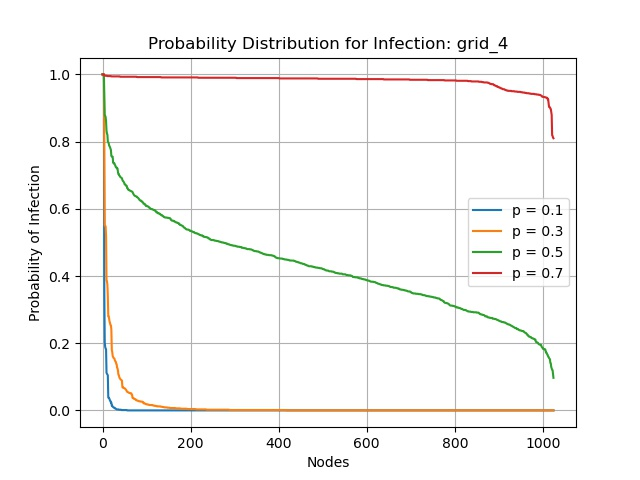
\includegraphics[width=0.9\textwidth]{pdist_grid_4.jpg}
        \caption{Probability Distributions $G^{4}_{gr}$}
        \label{fig:pdist_grid_1-jpg}
    \end{subfigure}
    \end{figure}

    The probability distributions for $G^{1}_{gr}$ and $G^{4}_{gr}$ seem to 
    follow the same pattern, but $G^{4}_{gr}$ has a slightly higher absolute
    probability of infection for the same number of nodes. This makes sense as
    the graphs are of the same general structure, so they scale similarly.

    \section{$G^{1}_{gr}$ and $G^{4}_{gr}$ Days to Infection Distribution}

    \begin{figure}[htpb]
        \centering
    \begin{subfigure}{.25\textwidth}
        \centering
        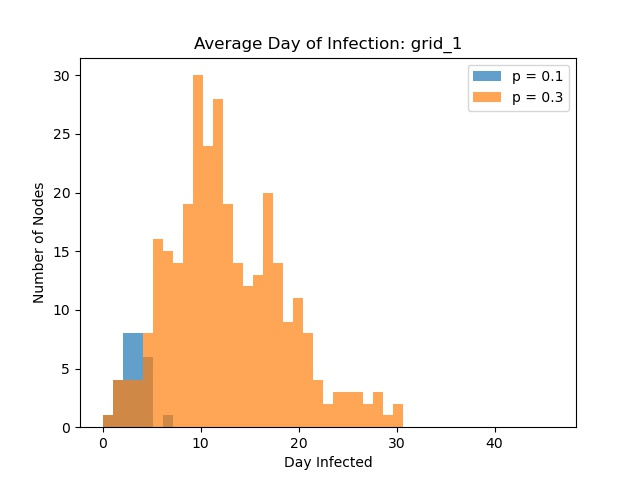
\includegraphics[width=0.25\textwidth]{histogram_grid_1_0_3.jpg}
        \caption{Day Infected $G^{1}_{gr}$}
        \label{fig:histogram_gr1_1_g}
    \end{subfigure}%
    \begin{subfigure}{.25\textwidth}
        \centering
        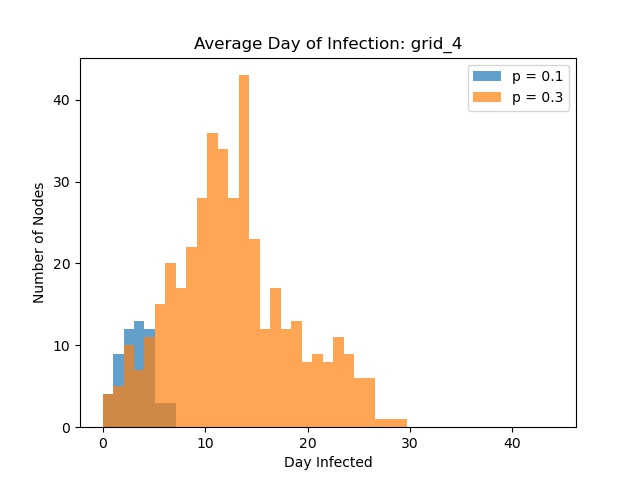
\includegraphics[width=0.25\textwidth]{histogram_grid_4_0_3.jpg}
        \caption{Day Infected $G^{4}_{gr}$}
        \label{fig:histogram_gr4_1_3}
    \end{subfigure}%
    %\end{figure}

    %\begin{figure}[htpb]
        %\centering
    \begin{subfigure}{.25\textwidth}
        \centering
        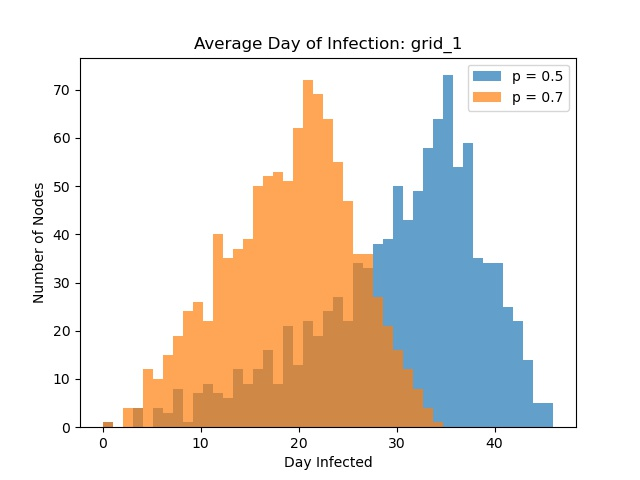
\includegraphics[width=0.25\textwidth]{histogram_grid_1_0_7.jpg}
        \caption{Day Infected $G^{1}_{gr}$}
        \label{fig:histogram_gr1_1_7}
    \end{subfigure}%
    \begin{subfigure}{.25\textwidth}
        \centering
        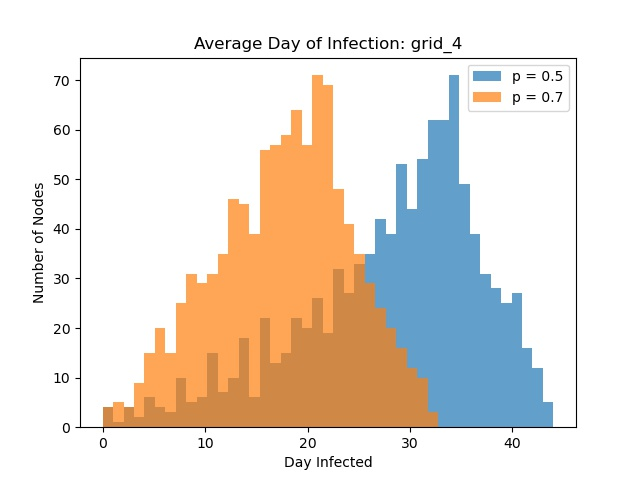
\includegraphics[width=0.25\textwidth]{histogram_grid_4_0_7.jpg}
        \caption{Day Infected $G^{4}_{gr}$}
        \label{fig:histogram_gr4_1_7}
    \end{subfigure}
    \end{figure}

    \begin{figure}[htp]
        \centering
        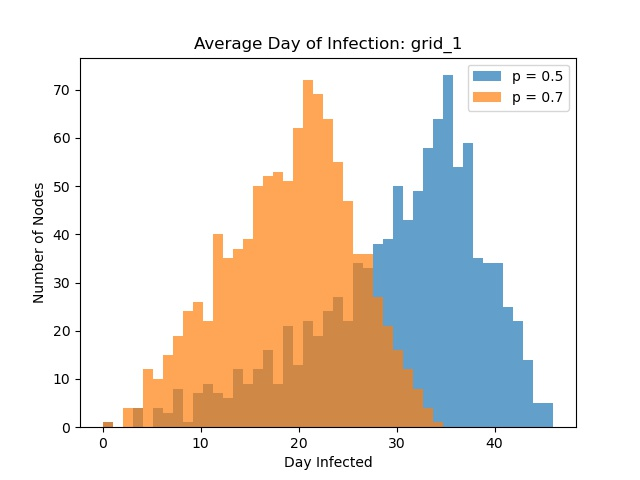
\includegraphics[width=0.3\textwidth]{histogram_grid_1_0_7.jpg}
        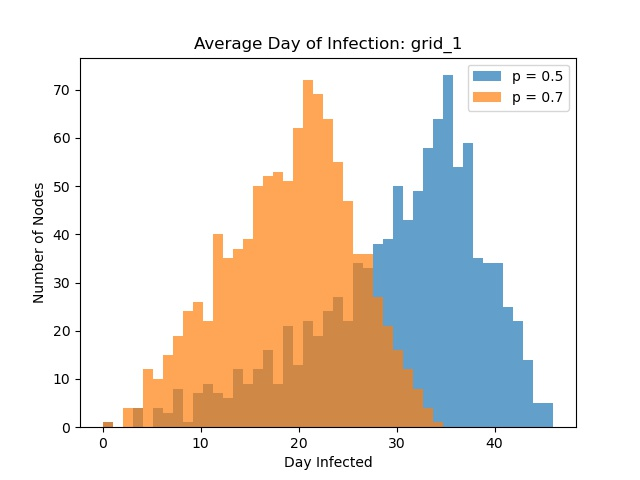
\includegraphics[width=0.3\textwidth]{histogram_grid_1_0_7.jpg}
        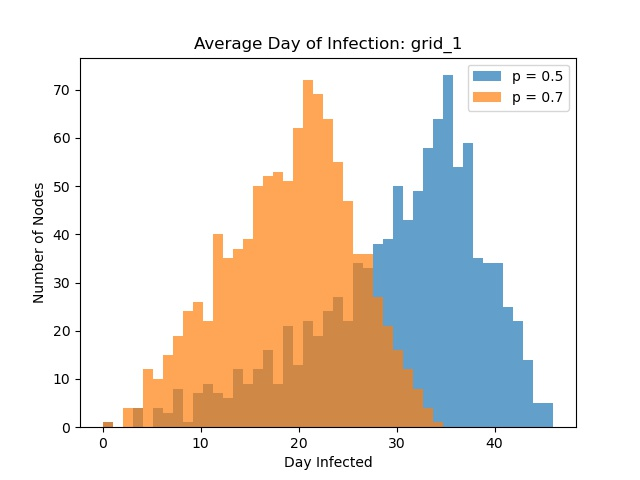
\includegraphics[width=0.3\textwidth]{histogram_grid_1_0_7.jpg}
    \end{figure}

    \begin{figure}[htp]
        \centering
        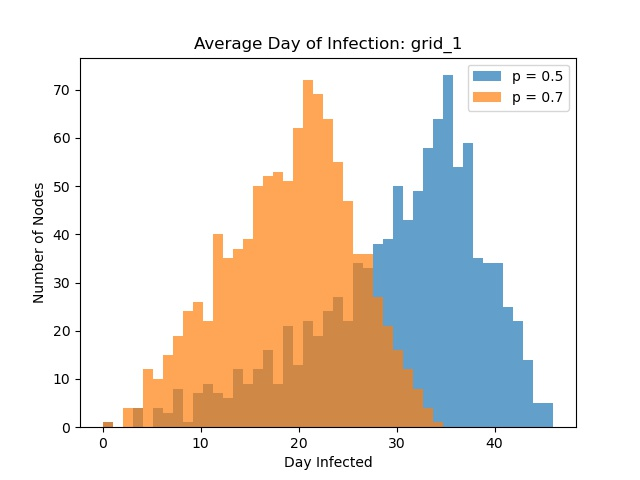
\includegraphics[width=0.25\textwidth]{histogram_grid_1_0_7.jpg}\hfill
        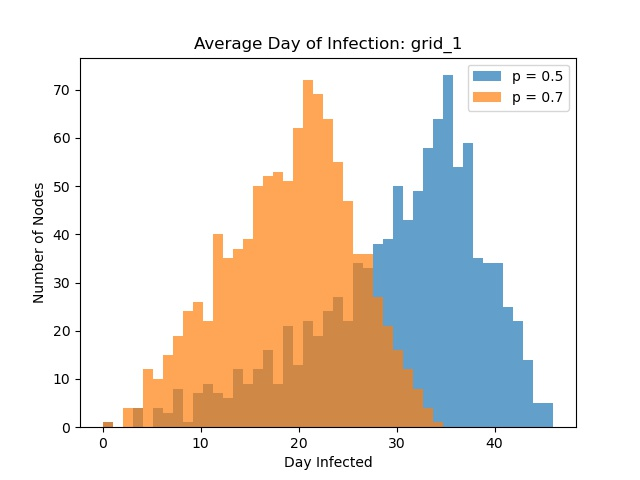
\includegraphics[width=0.25\textwidth]{histogram_grid_1_0_7.jpg}\hfill
        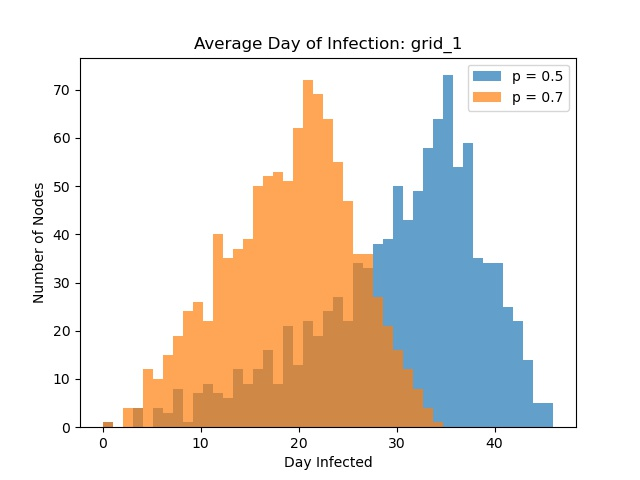
\includegraphics[width=0.25\textwidth]{histogram_grid_1_0_7.jpg}\hfill
        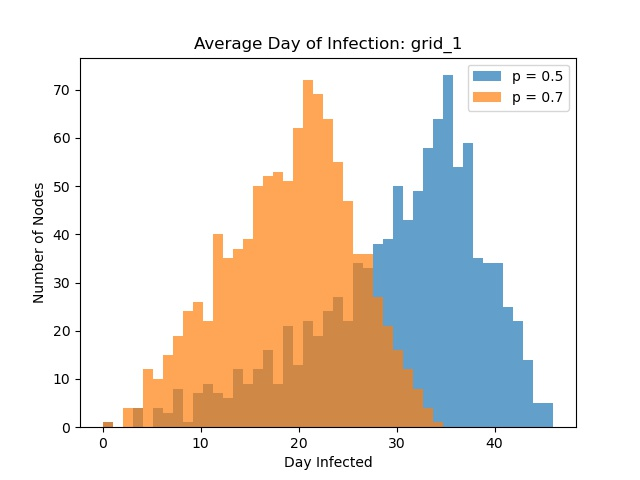
\includegraphics[width=0.25\textwidth]{histogram_grid_1_0_7.jpg}
    \end{figure}
testestslsdkfjlsdk

testestslsdkfjlsdk

lskdflsdkfj


lsdkflsdfjs

lsdkflsdkfj


\end{document}

